% Options for packages loaded elsewhere
\PassOptionsToPackage{unicode}{hyperref}
\PassOptionsToPackage{hyphens}{url}
%
\documentclass[
]{article}
\usepackage{lmodern}
\usepackage{amssymb,amsmath}
\usepackage{ifxetex,ifluatex}
\ifnum 0\ifxetex 1\fi\ifluatex 1\fi=0 % if pdftex
  \usepackage[T1]{fontenc}
  \usepackage[utf8]{inputenc}
  \usepackage{textcomp} % provide euro and other symbols
\else % if luatex or xetex
  \usepackage{unicode-math}
  \defaultfontfeatures{Scale=MatchLowercase}
  \defaultfontfeatures[\rmfamily]{Ligatures=TeX,Scale=1}
\fi
% Use upquote if available, for straight quotes in verbatim environments
\IfFileExists{upquote.sty}{\usepackage{upquote}}{}
\IfFileExists{microtype.sty}{% use microtype if available
  \usepackage[]{microtype}
  \UseMicrotypeSet[protrusion]{basicmath} % disable protrusion for tt fonts
}{}
\makeatletter
\@ifundefined{KOMAClassName}{% if non-KOMA class
  \IfFileExists{parskip.sty}{%
    \usepackage{parskip}
  }{% else
    \setlength{\parindent}{0pt}
    \setlength{\parskip}{6pt plus 2pt minus 1pt}}
}{% if KOMA class
  \KOMAoptions{parskip=half}}
\makeatother
\usepackage{xcolor}
\IfFileExists{xurl.sty}{\usepackage{xurl}}{} % add URL line breaks if available
\IfFileExists{bookmark.sty}{\usepackage{bookmark}}{\usepackage{hyperref}}
\hypersetup{
  pdftitle={Chapter 1 - Linear Models},
  pdfauthor={Weber Jakob},
  hidelinks,
  pdfcreator={LaTeX via pandoc}}
\urlstyle{same} % disable monospaced font for URLs
\usepackage[margin=1in]{geometry}
\usepackage{color}
\usepackage{fancyvrb}
\newcommand{\VerbBar}{|}
\newcommand{\VERB}{\Verb[commandchars=\\\{\}]}
\DefineVerbatimEnvironment{Highlighting}{Verbatim}{commandchars=\\\{\}}
% Add ',fontsize=\small' for more characters per line
\usepackage{framed}
\definecolor{shadecolor}{RGB}{248,248,248}
\newenvironment{Shaded}{\begin{snugshade}}{\end{snugshade}}
\newcommand{\AlertTok}[1]{\textcolor[rgb]{0.94,0.16,0.16}{#1}}
\newcommand{\AnnotationTok}[1]{\textcolor[rgb]{0.56,0.35,0.01}{\textbf{\textit{#1}}}}
\newcommand{\AttributeTok}[1]{\textcolor[rgb]{0.77,0.63,0.00}{#1}}
\newcommand{\BaseNTok}[1]{\textcolor[rgb]{0.00,0.00,0.81}{#1}}
\newcommand{\BuiltInTok}[1]{#1}
\newcommand{\CharTok}[1]{\textcolor[rgb]{0.31,0.60,0.02}{#1}}
\newcommand{\CommentTok}[1]{\textcolor[rgb]{0.56,0.35,0.01}{\textit{#1}}}
\newcommand{\CommentVarTok}[1]{\textcolor[rgb]{0.56,0.35,0.01}{\textbf{\textit{#1}}}}
\newcommand{\ConstantTok}[1]{\textcolor[rgb]{0.00,0.00,0.00}{#1}}
\newcommand{\ControlFlowTok}[1]{\textcolor[rgb]{0.13,0.29,0.53}{\textbf{#1}}}
\newcommand{\DataTypeTok}[1]{\textcolor[rgb]{0.13,0.29,0.53}{#1}}
\newcommand{\DecValTok}[1]{\textcolor[rgb]{0.00,0.00,0.81}{#1}}
\newcommand{\DocumentationTok}[1]{\textcolor[rgb]{0.56,0.35,0.01}{\textbf{\textit{#1}}}}
\newcommand{\ErrorTok}[1]{\textcolor[rgb]{0.64,0.00,0.00}{\textbf{#1}}}
\newcommand{\ExtensionTok}[1]{#1}
\newcommand{\FloatTok}[1]{\textcolor[rgb]{0.00,0.00,0.81}{#1}}
\newcommand{\FunctionTok}[1]{\textcolor[rgb]{0.00,0.00,0.00}{#1}}
\newcommand{\ImportTok}[1]{#1}
\newcommand{\InformationTok}[1]{\textcolor[rgb]{0.56,0.35,0.01}{\textbf{\textit{#1}}}}
\newcommand{\KeywordTok}[1]{\textcolor[rgb]{0.13,0.29,0.53}{\textbf{#1}}}
\newcommand{\NormalTok}[1]{#1}
\newcommand{\OperatorTok}[1]{\textcolor[rgb]{0.81,0.36,0.00}{\textbf{#1}}}
\newcommand{\OtherTok}[1]{\textcolor[rgb]{0.56,0.35,0.01}{#1}}
\newcommand{\PreprocessorTok}[1]{\textcolor[rgb]{0.56,0.35,0.01}{\textit{#1}}}
\newcommand{\RegionMarkerTok}[1]{#1}
\newcommand{\SpecialCharTok}[1]{\textcolor[rgb]{0.00,0.00,0.00}{#1}}
\newcommand{\SpecialStringTok}[1]{\textcolor[rgb]{0.31,0.60,0.02}{#1}}
\newcommand{\StringTok}[1]{\textcolor[rgb]{0.31,0.60,0.02}{#1}}
\newcommand{\VariableTok}[1]{\textcolor[rgb]{0.00,0.00,0.00}{#1}}
\newcommand{\VerbatimStringTok}[1]{\textcolor[rgb]{0.31,0.60,0.02}{#1}}
\newcommand{\WarningTok}[1]{\textcolor[rgb]{0.56,0.35,0.01}{\textbf{\textit{#1}}}}
\usepackage{graphicx}
\makeatletter
\def\maxwidth{\ifdim\Gin@nat@width>\linewidth\linewidth\else\Gin@nat@width\fi}
\def\maxheight{\ifdim\Gin@nat@height>\textheight\textheight\else\Gin@nat@height\fi}
\makeatother
% Scale images if necessary, so that they will not overflow the page
% margins by default, and it is still possible to overwrite the defaults
% using explicit options in \includegraphics[width, height, ...]{}
\setkeys{Gin}{width=\maxwidth,height=\maxheight,keepaspectratio}
% Set default figure placement to htbp
\makeatletter
\def\fps@figure{htbp}
\makeatother
\setlength{\emergencystretch}{3em} % prevent overfull lines
\providecommand{\tightlist}{%
  \setlength{\itemsep}{0pt}\setlength{\parskip}{0pt}}
\setcounter{secnumdepth}{-\maxdimen} % remove section numbering
\usepackage{amsmath}
\uspa

\title{Chapter 1 - Linear Models}
\author{Weber Jakob}
\date{}

\begin{document}
\maketitle

\begin{Shaded}
\begin{Highlighting}[]
\KeywordTok{library}\NormalTok{(gamair)}
\end{Highlighting}
\end{Shaded}

The classical data fitting process starts with the famous linear model:
\begin{equation}
  \label{eq:1}
   y_i = \beta x_i + \epsilon_i, \quad i=1, ..., n \qquad \qquad (1.1)
\end{equation} It is clear, that not all measured data is fit by this
model. Given some variability, what can be inferred from these data? In
particular:

\begin{enumerate}
\def\labelenumi{\arabic{enumi}.}
\tightlist
\item
  What value of \(\beta\) is the most consistent with the data?
\item
  What range of \(\beta\) is consistent with the data?
\item
  Are some particular theoretically derived values of \(\beta\)
  consistent with the data?
\end{enumerate}

These questions are answered by the statistical linear model.

\hypertarget{a-simple-linear-model}{%
\subsection{1.1 A simple linear model}\label{a-simple-linear-model}}

This section develops statistical methods for a simple linear model of
the form (1.1). Formally, consider \(n\) observations, \(x_i, y_i\),
where \(y_i\) is an observation on random variable, \(Y_i\), with
expectation, \(\mu_i = \mathbb{E}(Y_i)\). Suppose that an appropriate
model for the relationship between \(x\) and \(y\) is \begin{equation}
  Y_i = \mu_i + \epsilon_i, \quad \ where \ \mu_i = x_i \beta
\end{equation} Here, \(\beta\) is the unknown parameter and the
\(\epsilon_i\) are mutually independet zero mean random variables, each
with the same variance \(\sigma^2\). \(Y\) is an example of a
\emph{response variable}, while \(x\) is an example of a \emph{predictor
variable}. Such model is depicted in the following figure.
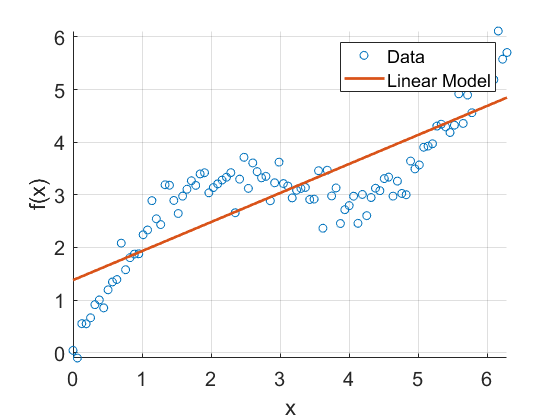
\includegraphics{images/cha1/lin_model.png}

\hypertarget{simple-least-squares-estimation}{%
\subsubsection{Simple least squares
estimation}\label{simple-least-squares-estimation}}

The basic approach to choose \(\beta\) is using the \emph{linear least
squares method}, which minimizes the sum of squared error between the
model output and the data. To do this, differentiate with respect to the
variable (here \(\beta\)) and set it to zero. This leads to the
\emph{least squares estimate} of \(\beta\): \begin{equation}
  \hat \beta = \sum_{i=1}^n x_i y_i / \sum_{i=1}^n x_i^2
\end{equation}

\hypertarget{sampling-properties-of-hat-beta}{%
\subsubsection{\texorpdfstring{1.1.1 Sampling properties of
\(\hat \beta\)}{1.1.1 Sampling properties of \textbackslash hat \textbackslash beta}}\label{sampling-properties-of-hat-beta}}

To evaluate the reliability of \(\beta\), we should consider some
properties of the distribution of \(\hat \beta\) values, which would be
obtained from repeated independet replication of the \(x_i, y_i\) data
used for estimation. Here the concept of an \emph{estimator} is
introduced, which is obtained by replacing the obersvations \(y_i\) in
the estimate of \(\hat \beta\) by the random variables, \(Y_i\).
Therefore, the \emph{estimator}, \(\hat \beta\) is a random variable.
The distribution of this random variable can now be discussed. Consider
only the first two moments of that distribution.\\
The expected value is \(\mathbb{E}(\hat \beta) = \beta\). So,
\(\hat \beta\) is an unbiased estimator (== its expected value is equal
to the true value of the parameter that it is supposed to estimate).\\
The variability is
\(var(\hat \beta) = (\sum_{i=1}^n x_i^2)^{-1} \sigma^2\). In most
circumstances, \(\sigma^2\) itself is an unknown parameter and must also
be estimated.

\hypertarget{how-old-is-the-universe}{%
\subsubsection{1.1.2 How old is the
universe?}\label{how-old-is-the-universe}}

\begin{Shaded}
\begin{Highlighting}[]
\KeywordTok{data}\NormalTok{(hubble)}
\NormalTok{hub.mod \textless{}{-}}\StringTok{ }\KeywordTok{lm}\NormalTok{(y}\OperatorTok{\textasciitilde{}}\NormalTok{x}\DecValTok{{-}1}\NormalTok{, }\DataTypeTok{data=}\NormalTok{hubble)}
\KeywordTok{summary}\NormalTok{(hub.mod)}
\end{Highlighting}
\end{Shaded}

\begin{verbatim}
## 
## Call:
## lm(formula = y ~ x - 1, data = hubble)
## 
## Residuals:
##    Min     1Q Median     3Q    Max 
## -736.5 -132.5  -19.0  172.2  558.0 
## 
## Coefficients:
##   Estimate Std. Error t value Pr(>|t|)    
## x   76.581      3.965   19.32 1.03e-15 ***
## ---
## Signif. codes:  0 '***' 0.001 '**' 0.01 '*' 0.05 '.' 0.1 ' ' 1
## 
## Residual standard error: 258.9 on 23 degrees of freedom
## Multiple R-squared:  0.9419, Adjusted R-squared:  0.9394 
## F-statistic: 373.1 on 1 and 23 DF,  p-value: 1.032e-15
\end{verbatim}

\begin{Shaded}
\begin{Highlighting}[]
\KeywordTok{plot}\NormalTok{(}\KeywordTok{fitted}\NormalTok{(hub.mod), }\KeywordTok{residuals}\NormalTok{(hub.mod), }\DataTypeTok{xlab=}\StringTok{"fitted values"}\NormalTok{, }\DataTypeTok{ylab =} \StringTok{"residuals"}\NormalTok{)}
\end{Highlighting}
\end{Shaded}

\includegraphics{Chapter1_LinearModels_files/figure-latex/Age of the universe-1.pdf}
The plot of fitted values (\(\mu_i = \beta x_i\)) vs.~residuals
(\(\epsilon_i = y_i - \mu_i\)) checks the assumption of random noise
with zero mean. The plot should show an apparently random scatter of
residuals around zero.

\hypertarget{adding-a-distributional-assumption}{%
\subsubsection{1.1.3 Adding a distributional
assumption}\label{adding-a-distributional-assumption}}

Further distributional assumptions are necessary to find confidence
intervals for \(\beta\), or test hypotheses related to the model.
Specifically, assume that \(\epsilon_i \sim \mathcal{N}(0, \sigma^2)\)
for all i, which is equivalent to assuming
\(Y_i \sim \mathcal{N}(x_i\beta, \sigma^2)\). We have already seen that
\(\hat \beta\) is just a weighted sum of \(Y_i\), which itself is a
random variable. This makes \(\hat \beta\) a random variable. Therefore,
we have \[
  \hat \beta \sim \mathcal{N}\big( \beta, (\sum x_i^2)^{-1} \sigma^2\big)  \qquad \qquad (1.4)
\] \textbf{Testing hypotheses about \(\beta\)}\\
Here, classic hypothesis testing is introduce: We can test the null
hypothesis, \(H_0 : \beta = \beta_0\), versus the alternative
hypothesis, \(H_1 : \beta \neq \beta_0\), for some specified value
\(\beta_0\), by examining the probability of getting the observed
\(\hat \beta\) assuming \(H_0\) to be true. If \(\sigma^2\) were known
we could work directly with (1.4), as follows. The probability required
is known as \emph{p-value} of the test. It is the probability of getting
a value of \(\hat \beta\) at least as favourable to \(H_1\) as the one
actually observed, if \(H_0\) is actually true. The p-value is the \[
  p = P\Big[ \frac{\vert \hat \beta - \beta_0 \vert}{\sigma_{\hat \beta}} \ge \frac{\vert \hat \beta_{obs} - \beta_0 \vert}{\sigma_{\hat \beta}}\Big \vert H_0 \Big] = P\Big[ \vert Z \vert \ge \vert z \vert \Big]
\] where \(\hat \beta_{obs}\) is the estimate, \(\hat \beta\) is the
estimator, \(Z \sim \mathcal N(0,1)\),
\(z = (\hat \beta_{obs} - \beta_0)/\sigma_{\hat \beta}\) and
\(\sigma_{\hat \beta} = (\sum x_i^2)^{-1} \sigma^2\). Hence, having
formed Z, the p-value is easily worked out using the cumulative
distribution functionfor the standard normal. Small p-values suggest
that the data are inconsistent with \(H_0\), while large values indicate
consistency. In reality \(\sigma^2\) is usually unknown. Therefore,
\(\sigma\) is replaced by \(\hat \sigma\). This introduces some extra
uncertainty (unless the sample size is very large). It turns out that if
\(H_0 : \beta = \beta_0\) is true then \[
  T \equiv \frac{\hat \beta - \beta_0}{\sigma_{\hat \beta}} \sim t_{n-1}
\] where \(n\) is the sample size and \(t_{n-1}\) is the
\emph{t-distribution} with \(n-1\) degrees of freedom. Large magnitude
values of T favour \(H_1\), so using T as the test statistic, in place
of \(\hat \beta\) we can calulate the p-value by evaluating \[
  p = P\Big[\vert T \vert > \vert t \vert \Big]
\] where \(T \sim t_{n-1}\) and
\(t = (\hat \beta_{obs} - \beta_0)/ \sigma_{\hat \beta}\). Here is some
code to evaluate the p-value for \(H_0 : \beta = 163000000\)

\begin{Shaded}
\begin{Highlighting}[]
\NormalTok{cs.hubble \textless{}{-}}\StringTok{ }\DecValTok{163000000}
\NormalTok{t.stat \textless{}{-}}\StringTok{ }\NormalTok{(}\KeywordTok{coef}\NormalTok{(hub.mod) }\OperatorTok{{-}}\StringTok{ }\NormalTok{cs.hubble) }\OperatorTok{/}\StringTok{ }\KeywordTok{summary}\NormalTok{(hub.mod)}\OperatorTok{$}\NormalTok{coefficients[}\DecValTok{2}\NormalTok{]}
\KeywordTok{pt}\NormalTok{(t.stat, }\DataTypeTok{df=}\DecValTok{23}\NormalTok{)}\OperatorTok{*}\DecValTok{2}
\end{Highlighting}
\end{Shaded}

\begin{verbatim}
##             x 
## 5.688416e-161
\end{verbatim}

As judged by the test statistic, \(t\), the data would be hugely
improbably if \(\beta = 1.63*10^8\).

Hypothesis testing is usefull when there are good reasons to want to
stick with some null hypothesis, until there is good reason to reject
it.

\textbf{Confidence intervals}\\
The natural question after testing whether a particular value of
\(\beta\) is consistent with the data, is \emph{what range} of values of
\(\beta\) would be consistent with the data. To do this, we need a
definition of ``consistent'': a common choice is to say that any
parameter value is consistent with the data if it results in a p-value
of \(\ge 0.05\), when used as the null value in a hypothesis test.\\
The defining property of a 95\% confidence interval is this: if we were
to gather an infinite sequence of independent replicate data sets, and
calulate 95\% confidence intervals for \(\beta\) from each, then 95\% of
these intervals would include the true \(\beta\), and 5\% would not. For
the hubble example, a 95\% CI for the hubble constant is given by:

\begin{Shaded}
\begin{Highlighting}[]
\NormalTok{sigb \textless{}{-}}\StringTok{ }\KeywordTok{summary}\NormalTok{(hub.mod)}\OperatorTok{$}\NormalTok{coefficients[}\DecValTok{2}\NormalTok{]}
\NormalTok{h.ci \textless{}{-}}\StringTok{ }\KeywordTok{coef}\NormalTok{(hub.mod) }\OperatorTok{+}\StringTok{ }\KeywordTok{qt}\NormalTok{(}\KeywordTok{c}\NormalTok{(}\FloatTok{0.025}\NormalTok{, }\FloatTok{0.975}\NormalTok{), }\DataTypeTok{df=}\DecValTok{21}\NormalTok{) }\OperatorTok{*}\StringTok{ }\NormalTok{sigb}
\CommentTok{\# now construct the confidence interval}
\NormalTok{h.ci \textless{}{-}}\StringTok{ }\NormalTok{h.ci}\OperatorTok{*}\DecValTok{60}\OperatorTok{\^{}}\DecValTok{2}\OperatorTok{*}\DecValTok{24}\OperatorTok{*}\FloatTok{365.25}\OperatorTok{/}\FloatTok{3.09e19} \CommentTok{\# convert to 1/years}
\KeywordTok{sort}\NormalTok{(}\DecValTok{1}\OperatorTok{/}\NormalTok{h.ci)}
\end{Highlighting}
\end{Shaded}

\begin{verbatim}
## [1] 11543125363 14328653915
\end{verbatim}

Actually this ``Hubble age'' is the age of the universe if it has been
expanding freely, essentially unfettered by gravitation. If the universe
is really `matter dominated' then the galaxies should be slowed by
gravity over time so that the universe would actually be younger than
this, but it is time to get on with the subject of this book.

\end{document}
